\chapter{Thực nghiệm và thảo luận}
\section{Các tập đánh giá và đơn vị báo cáo}
\begin{table}[htbp]\centering\small
\caption{Phạm vi các phép đo tracking. Thời gian chờ được biểu diễn bằng số bước ở tốc độ của từng tập.}\label{tab:splits}
\begin{tabular}{lrrrl}\hline
Tập & Chuỗi & Khung hình & fps & Chờ\\\hline
UA-DETRAC test40 & 40 & 56.340 & 25 & 30 bước\\
BDD100K MOT val & 200 & 39.973 & 5 & 6 bước\\
SVMOT test & 9 & 8.250 & 30 & 36 bước\\
SVMOT bổ sung & 21 & 18.650 & 30 & 36 bước\\
RoundaboutHD phần đầu & 4 & 12.000 & 15 & 18 bước\\
RoundaboutHD phần mở rộng & 4 & 24.000 & 15 & 18 bước\\
Sherbrooke cars ROI & 1 & 1.001 & 30 & 36 bước\\
HELMET test & 182 & 18.200 & 10 & 12 bước\\
UTUAV B/C validation & 2 & 1.489 & 29,97 & 36 bước\\\hline
\end{tabular}
\end{table}
Trên UA-DETRAC, phép đo detector chỉ báo AP cho ô tô và xe buýt. Các vùng \emph{van}, \emph{others} và vùng bỏ qua không tham gia như nhãn dương của hai lớp đó. Có 173 ảnh thiếu phần tử khung hình trong XML nên còn 56.167 ảnh khi chấm detector. Trong phép đo tracking, bộ chấm dùng danh tính phương tiện gộp, kể cả \emph{van} và \emph{others}. Toàn bộ 56.340 ảnh vẫn đi qua đường theo dõi. Trên 173 ảnh nói trên, bộ chấm coi GT trống. Chưa đủ bằng chứng để coi mọi xe xuất hiện ở đó là phát hiện nhầm trong thế giới thực.

BDD val dùng nhãn COCO-video cho năm lớp và xử lý vùng crowd theo bộ chấm của dự án. Có 615 ảnh không có chú thích được giữ trong dòng thời gian. BDD val đã được quan sát trong quá trình phát triển, nên mức độ độc lập của tập này khác với một tập kiểm tra kín. SVMOT và RoundaboutHD chỉ có lần lượt hai cảnh và bốn camera của cùng một nút giao. Vì thế hai phép đánh giá ngoài chỉ báo kết quả mô tả. Một điểm HOTA cao hơn giữa hai tập có thể phản ánh quy tắc chấm, mật độ nhãn hoặc tốc độ lấy mẫu khác nhau.

HELMET được chấm trên toàn bộ test chính thức. Trong đó, 36 clip từng dùng để đánh giá ban đầu được đối chiếu lại và 146 clip còn lại được báo riêng để kiểm tra tính nhất quán. UTUAV được dùng để khảo sát giới hạn chuyển miền sang góc nhìn UAV trong hai block B và C. Các phép đo ngoài phục vụ những kịch bản riêng, với đơn vị nhãn và quy tắc đánh giá theo từng tập.

\section{Bộ phát hiện trước và sau tinh chỉnh}
\begin{table}[htbp]\centering\small
\caption{mAP của ba checkpoint trên thang 0--1. UA tính trên hai lớp, BDD tính trên năm lớp. Nguồn R53.}\label{tab:ap}
\begin{tabular}{lrrrr}\hline
& \multicolumn{2}{c}{UA-DETRAC test} & \multicolumn{2}{c}{BDD100K val}\\
Detector & 50 & 50--95 & 50 & 50--95\\\hline
YOLOv8n COCO & 0,8701 & 0,5997 & 0,2439 & 0,1571\\
YOLOv8n mixed5 & 0,8785 & 0,6111 & 0,3896 & 0,2544\\
YOLO11n mixed5 & 0,8884 & 0,6222 & 0,3787 & 0,2494\\\hline
\end{tabular}
\end{table}
Trên UA-DETRAC, YOLO11n mixed5 có mAP50 cao nhất trong ba checkpoint. Điểm trung bình che một khác biệt theo lớp. AP50 ô tô tăng từ 0,8577 ở YOLOv8n COCO lên 0,9055 ở YOLO11n mixed5, trong khi AP50 xe buýt giảm từ 0,8825 xuống 0,8713. Do đó, lựa chọn detector dựa trên mAP có thể khác lựa chọn của một ứng dụng chuyên theo dõi xe buýt.

Trên BDD val, YOLOv8n mixed5 cho mAP50 cao nhất. Đối với xe máy, AP50 tăng từ 0,1175 lên 0,2174 khi so hai cấu hình YOLOv8n. Dù vậy, recall vận hành của YOLOv8n mixed5 ở lớp xe máy chỉ đạt 0,2284 trên 902 hộp có nhãn, thấp hơn nhiều so với 0,7040 trên 341.436 hộp ô tô. Một bộ lọc phía sau detector chỉ có thể nối các quan sát thưa nếu quỹ đạo đã hình thành và thời gian chờ còn hiệu lực. Kết quả AP là ước lượng điểm; chưa có khoảng tin cậy AP cho test40 và BDD val.

Checkpoint YOLO11n 50/50 dùng trong phép đo Nano được kiểm tra riêng tại kích thước $384\times640$ trên PC. Trên BDD val, mô hình đạt mAP50 37,89\%, mAP50--95 24,74\% và AP50 xe máy 21,14\%. Trên UA-DETRAC test40, mAP50 của ô tô và xe buýt là 89,08\% và mAP50--95 là 62,40\%. Tương ứng, AP50 riêng của ô tô và xe buýt là 90,55\% và 87,60\%. Các điểm này đánh giá checkpoint 50/50 trên PC. Chất lượng tracking từ engine FP16 thực tế được chấm riêng trên các đoạn xử lý ở Chương~\ref{chap:nano}.

\begin{table}[htbp]\centering\small
\caption{Độ chính xác từng lớp của YOLO11n 50/50 trên BDD100K val. Các chỉ số theo phần trăm. Precision và recall ở ngưỡng vận hành 0,25. Nguồn R108.}\label{tab:ap-classes}
\begin{tabular}{lrrrrr}\toprule
Lớp & Hộp GT & AP50 & AP50--95 & Precision & Recall\\\midrule
Ô tô & 341.436 & 77,21 & 51,10 & 83,71 & 67,84\\
Xe tải & 27.343 & 37,62 & 26,74 & 70,25 & 31,40\\
Xe buýt & 9.087 & 36,74 & 27,95 & 58,97 & 34,47\\
Xe máy & 902 & 21,14 & 9,91 & 22,16 & 29,60\\
Xe đạp & 4.135 & 16,75 & 7,99 & 50,39 & 12,65\\\bottomrule
\end{tabular}
\end{table}
Độ lệch số lượng nhãn giữa các lớp đòi hỏi báo cáo AP riêng. Với checkpoint 50/50, lớp xe máy có recall cao hơn YOLO11n mixed5 ban đầu trong điểm vận hành đã đo, đồng thời precision thấp hơn. Điểm AP phản ánh nhiều ngưỡng điểm, còn một cấu hình tracking cụ thể chỉ nhận các hộp sau ngưỡng đã chọn. Chất lượng trên BDD vì vậy được báo cùng ma trận tracking khi detector bị cố định.

\section{Giữ ID khi cua và khi bị che}
Phép thử trên 12 video phát triển UA-DETRAC dùng YOLOv8n COCO ở ngưỡng trên 0,25. KF/CV đạt 59,00 HOTA, EKF 59,25 và UKF 58,79 trên thang 100. Khoảng tin cậy cho hiệu HOTA của từng cấu hình EKF và UKF so với CV đều chứa 0. PF100 đạt 49,33. Biến thể PF100 với phân bố đề xuất có dùng phép đo (K1) đạt 53,77. Đây là phép khảo sát trên tập phát triển với 100 hạt, tách biệt với benchmark 500 hạt ở các phần sau.

Phân tích che khuất bắt đầu với 717 sự kiện. Chỉ 184 sự kiện trên 137 quỹ đạo có đủ GT trước và sau để đánh giá việc nối ID. Trong 33 sự kiện che gần hoàn toàn trên sáu video, tỷ lệ giữ ID của các biến thể chỉ khoảng 0,02--0,09. Các khoảng tin cậy cho hiệu số đều chứa 0. Nếu tính cả trường hợp xe đã ra khỏi vùng có nhãn vào mẫu số, kết quả sẽ trộn mất ID với mất khả năng quan sát danh tính chuẩn.

Trong 1.185 quỹ đạo GT trên tập phát triển, tiêu chí dựa trên độ cong cực đại nhận được 32 quỹ đạo cua ở năm video. Khi dùng phân vị 90 thay cho cực đại, chỉ còn tám quỹ đạo ở bốn video. Tầng thứ hai chỉ dùng để đếm mẫu. Trên tầng thứ nhất, PF100 giữ ID kém hơn EKF. Không thể từ đây suy ra mô hình nào tốt nhất cho riêng xe máy rẽ. Cả nhãn loại xe lẫn số quỹ đạo cua có thể kiểm tra đều giới hạn câu trả lời.

\section{UA-DETRAC test40}
\begin{table}[htbp]\centering\small
\caption{HOTA COMBINED trên UA-DETRAC test40, thang 100. PF500 là trung bình điểm của ba seed. Nguồn R56.}\label{tab:ua}
\begin{tabular}{llrrrr}\hline
Detector & Ngưỡng & CV & EKF & UKF & PF500\\\hline
YOLOv8n COCO & c25 & 58,235 & 58,353 & 58,244 & 55,080\\
YOLOv8n COCO & c10 & 57,969 & 58,303 & 58,154 & 55,069\\
YOLOv8n mixed5 & c25 & 61,643 & 61,711 & 61,630 & 58,545\\
YOLOv8n mixed5 & c10 & 61,243 & 61,426 & 61,293 & 58,276\\
YOLO11n mixed5 & c25 & 62,063 & 62,239 & 62,181 & 58,811\\
YOLO11n mixed5 & c10 & 61,531 & 61,794 & 61,729 & 58,599\\
\hline\end{tabular}\end{table}

Đọc theo một hàng của Bảng~\ref{tab:ua} giữ được cùng phát hiện cho cả bốn bộ lọc. Trong nhóm YOLO11n mixed5 c25, EKF đạt 62,239 HOTA và CV đạt 62,063. Hiệu 0,176 điểm nhỏ hơn nhiều so với mức giảm khi thay CV bằng PF500 trong cùng nhóm. Khi giữ CV và đổi detector ở c25, điểm thay đổi từ 58,235 với YOLOv8n COCO lên 62,063 với YOLO11n mixed5. Phép so thứ hai cho thấy độ lớn của thay đổi cấu hình detector, nhưng thiết kế không có CI cho hiệu giữa detector.

Trên cả sáu hàng, độ chênh giữa CV, EKF và UKF tối đa 0,34 điểm HOTA. CI 95\% cho hiệu EKF trừ CV không chứa 0 ở hai trong sáu nhóm, gồm YOLOv8n COCO c10 và YOLO11n mixed5 c25. PF500 thấp hơn ba bộ lọc còn lại từ 2,90 đến 3,43 điểm HOTA trên các đối chứng của sáu nhóm. Các khoảng cho hiệu đó không chứa 0. Phân tích bootstrap được cố định sau khi đã xem điểm test40, nên các khoảng này có giá trị mô tả hậu nghiệm.

\subsection{Đối chứng với SORT}
Ở c25, sáu cặp cùng detector và cùng bộ lọc CV hoặc EKF cho HOTA ByteTrack cao hơn SORT từ 1,380 đến 3,714 điểm. Ví dụ với YOLOv8n COCO và CV, ByteTrack đạt 58,235 còn SORT đạt 54,521. IDSW giảm từ 4.318 xuống 2.498 nhưng FP tăng từ 62.846 lên 73.478. Trong cặp này, khả năng nối ID tốt hơn đi cùng nhiều hộp không khớp GT hơn. Chỉ số HOTA tổng hợp hai mặt của thay đổi đó.

Với YOLO11n mixed5 và CV, chênh HOTA chỉ còn 1,380 điểm. AssA tăng 2,921 điểm trong khi DetA giảm 0,060 điểm. Như vậy nguồn chênh chủ yếu nằm ở liên kết. Phép so chỉ thực hiện ở c25, nơi vòng ghép điểm thấp của ByteTrack rỗng. Khác biệt quan sát được thuộc về toàn bộ cơ chế ghép và quản lý vòng đời trong hai tracker. Không có CI cho sáu cặp này.

\section{BDD100K val}
\begin{table}[htbp]\centering\small
\caption{HOTA COMBINED trên BDD100K val, thang 100. PF500 là trung bình điểm của ba seed. Nguồn R61.}\label{tab:bdd}
\begin{tabular}{llrrrr}\hline
Detector & Ngưỡng & CV & EKF & UKF & PF500\\\hline
YOLOv8n COCO & c25 & 33,677 & 33,827 & 33,769 & 29,661\\
YOLOv8n COCO & c10 & 34,104 & 34,353 & 34,211 & 30,122\\
YOLOv8n mixed5 & c25 & 45,059 & 45,200 & 45,122 & 38,697\\
YOLOv8n mixed5 & c10 & 45,298 & 45,499 & 45,406 & 38,987\\
YOLO11n mixed5 & c25 & 44,856 & 45,061 & 44,955 & 38,620\\
YOLO11n mixed5 & c10 & 45,143 & 45,282 & 45,223 & 38,891\\
\hline\end{tabular}\end{table}

Điểm cao nhất trong ma trận thuộc YOLOv8n mixed5 c10 với EKF. Cấu hình này đạt HOTA 45,499, IDF1 55,170 và 11.067 lần đổi ID. So với CV trên cùng cache, hiệu HOTA là $+0{,}201$ điểm, CI 95\% từ $+0{,}081$ đến $+0{,}325$. Trong cùng nhóm, PF500 thấp hơn EKF 6,511 điểm với CI từ $-7{,}044$ đến $-5{,}980$. Hai cặp có độ lớn chênh rất khác nhau dù cùng được xét trên 200 video.

Trên cả sáu nhóm, EKF cao hơn CV về HOTA và sáu khoảng cho hiệu số đều nằm phía trên 0. Sáu khoảng UKF trừ CV đều chứa 0. PF500 thấp hơn các cấu hình còn lại về HOTA và IDF1 ở cả sáu nhóm. Việc chênh EKF và CV khá nhỏ nhưng khoảng nằm trên 0 trả lời câu hỏi về tính nhất quán trên mẫu video này. Mức chênh có đáng đổi cấu hình trong một ứng dụng cụ thể hay không còn phụ thuộc chi phí xử lý và yêu cầu về danh tính của ứng dụng.

\section{Chuyển sang cảnh và camera mới}
\subsection{SVMOT}
Bộ SVMOT có nhiều phương tiện dừng và nhiều trường hợp che khuất \cite{svmot}. Chín chuỗi test được ghi ở hai cảnh, bốn chuỗi buổi sáng và năm chuỗi buổi tối. Detector xử lý toàn ảnh theo giao thức dự án. Một xe xa nằm ngoài vùng có nhãn vẫn có thể bị tính FP. Ở c25 với YOLOv8n COCO, HOTA lần lượt là 48,66, 49,65, 49,21 và 50,70 cho CV, EKF, UKF và PF500. Tuy nhiên, khi tách theo cảnh, PF500 đạt 46,53 so với 46,78 của CV ở cảnh sáng, còn ở cảnh tối là 54,38 so với 50,39. Lợi thế tổng hợp của PF tập trung ở cảnh thứ hai. Chưa thể quy nguyên nhân cho ánh sáng vì cảnh quay và thời điểm thay đổi cùng nhau.

Ba seed PF500 trong nhóm này cho HOTA 51,30, 51,31 và 49,50. IDSW trung bình là 427,3 so với 407 của EKF. Có thể cải thiện HOTA dù còn nhiều lần đổi ID hơn vì HOTA cũng tính phát hiện và độ nhất quán liên kết trên toàn quỹ đạo. Với hai detector mixed5, DetA thấp hơn YOLOv8n COCO khoảng mười điểm. Không có CI trên hai cảnh và không dùng các điểm này để chọn lại checkpoint.

Phép kiểm che khuất gắn sự kiện với giá trị \emph{visibility} của hộp GT ở thời điểm đánh giá. Mức không quá 0,5 xác định nhóm che khuất trong Bảng~\ref{tab:svmot-vis}. Trong test chính thức, EKF có ít hơn KF mười lần đổi ID, còn UKF bằng KF. Trên 21 chuỗi thuộc split train chính thức, chiều chênh lệch đổi ID không lặp lại. Kết quả của 21 chuỗi được báo như một khảo sát mô tả riêng; điểm test chính thức giữ nguyên 9 chuỗi. Chênh lệch FN nhỏ trong từng nhóm cho phép đọc IDSW cùng với độ phủ mẫu.

\begin{table}[htbp]\centering\small
\caption{Kết quả SVMOT với YOLOv8n COCO c25 trên hai phần của bản phát hành.}\label{tab:svmot-vis}
\begin{tabularx}{\linewidth}{@{}Xrrrr@{}}\toprule
Phạm vi và chỉ số & Hộp GT & KF & EKF & UKF\\\midrule
9 chuỗi test, IDSW toàn phần & 70.220 & 435 & 407 & 418\\
9 chuỗi test, IDSW ở visibility $\leq0{,}5$ & 12.051 & 125 & 115 & 125\\
9 chuỗi test, FN ở visibility $\leq0{,}5$ & 12.051 & 6.515 & 6.517 & 6.497\\
21 chuỗi bổ sung, IDSW toàn phần & 173.242 & 1.189 & 1.162 & 1.162\\
21 chuỗi bổ sung, IDSW ở visibility $\leq0{,}5$ & 22.221 & 149 & 152 & 156\\
21 chuỗi bổ sung, FN ở visibility $\leq0{,}5$ & 22.221 & 12.637 & 12.630 & 12.626\\\bottomrule
\end{tabularx}
\end{table}

Trên test9, tỷ lệ hộp GT khả kiến thấp có ít nhất một phát hiện đạt IoU từ 0,5 tăng từ 49,03\% ở ngưỡng 0,25 lên 67,42\% ở ngưỡng 0,10. Đây là độ phủ ứng viên trước ghép một-một. Khi hạ ngưỡng, FN toàn video của KF giảm từ 14.665 xuống 12.924 và FP tăng từ 21.964 lên 29.836. Trong riêng nhóm đang che ở ngưỡng 0,10, IDSW là 105, 107 và 106 cho KF, EKF và UKF. Phép kiểm cho thấy sự đánh đổi giữa phục hồi quan sát và báo nhầm khi đưa thêm hộp vào ByteTrack.

\subsection{RoundaboutHD}
RoundaboutHD cung cấp nhãn cho cả bài toán đa camera và đơn camera \cite{round}. Giao thức lấy 3.000 khung liên tiếp đầu tiên của mỗi camera tại cùng một vòng xuyến. GT là quỹ đạo đơn camera trong SCT. Tám cặp hộp của ID 105 ở camera 4 trùng khóa khung--ID nhưng khác tọa độ. Quy trình bỏ cả 16 dòng liên quan ở các khung 2536--2543, giữ phần còn lại của quỹ đạo. Nhãn SCT không phủ các xe đỗ trong bãi. Một dự đoán đúng vị trí xe đỗ vẫn có thể bị tính FP. Quy tắc này ảnh hưởng trực tiếp đến cách diễn giải kết quả detector.

Với YOLOv8n mixed5 c25, CV đạt 42,83 HOTA, EKF đạt 42,48, UKF đạt 42,44 và PF500 chỉ đạt 31,27. Trên sáu nhóm, ba cấu hình đầu cách nhau tối đa 0,6 điểm. PF500 thấp hơn CV từ 11,56 đến 12,35 điểm ở COMBINED và có IDSW gấp 2,22 đến 2,91 lần. Chiều giảm xuất hiện trong đủ 72 tổ hợp camera, detector, ngưỡng và seed. Khác biệt này lớn hơn dao động giữa các seed. Bảng đầy đủ cho hai tập ngoài được trình bày ở Phụ lục~\ref{app:ho-so}.

\subsection{RoundaboutHD: đánh giá trên 24.000 khung tiếp theo}
Trong vòng mở rộng, mỗi camera dùng lại dự đoán detector của 3.000 khung đầu để tạo lịch sử tracker, rồi chạy tiếp đến khung 9.000. Bốn cấu hình dùng YOLOv8n COCO c25, chung giới hạn chờ 18 khung, với PF500 K1/K2 motion2 ở ba seed. Mốc rẽ được lấy từ GT trên toàn timeline. Tại mỗi khung, phương pháp lấy trung vị điểm giữa đáy hộp quanh ba mốc cách nhau 13 khung, rồi tính góc giữa hai vectơ dịch chuyển. Mỗi vectơ phải dài ít nhất $\max(8\,\text{px},0{,}25h)$, với $h$ là chiều cao hộp GT. Một đoạn rẽ yêu cầu ít nhất tám khung liên tiếp đạt ngưỡng và cùng chiều đổi hướng. Ngưỡng chính là $25^\circ$, ngưỡng $35^\circ$ dùng để kiểm tra độ nhạy, còn nhóm gần thẳng dùng tối đa $8^\circ$. Góc được đo trên ảnh và chịu ảnh hưởng của phối cảnh.

\begin{table}[htbp]\centering\small
\caption{Số lần đổi ID theo nhóm chuyển động trên phần mở rộng RoundaboutHD. PF là trung bình ba seed.}\label{tab:round-ext}
\begin{tabular}{@{}lrrrrr@{}}\toprule
Nhóm & Hộp GT & KF & EKF & UKF & PF500\\\midrule
Đổi hướng từ $25^\circ$ & 13.509 & 34 & 28 & 28 & 40,33\\
Đổi hướng từ $35^\circ$ & 8.659 & 29 & 24 & 24 & 33,00\\
Gần thẳng & 78.372 & 426 & 423 & 418 & 658,67\\
Toàn cửa sổ mới & 157.222 & 716 & 726 & 725 & 1.020,33\\\bottomrule
\end{tabular}
\end{table}
Với ngưỡng $25^\circ$, EKF và UKF cùng giảm 17,65\% IDSW so với KF. Số lượt bỏ sót tương ứng của KF, EKF và UKF là 5.275, 5.264 và 5.263. Mức giảm IDSW xuất hiện trên camera 1, 2 và 3. Ở camera 4, cả ba cấu hình đều có 10 lần đổi ID trong nhóm này. Khi xét từng đoạn, 645 trong 652 đoạn có cùng số lần đổi ID giữa ba bộ lọc. Cả EKF và UKF cùng cải thiện ở sáu đoạn và cùng tăng IDSW ở một đoạn. Hình~\ref{fig:trajectory-cases} minh họa một trường hợp của mỗi chiều thay đổi.

\begin{figure}[htbp]\centering
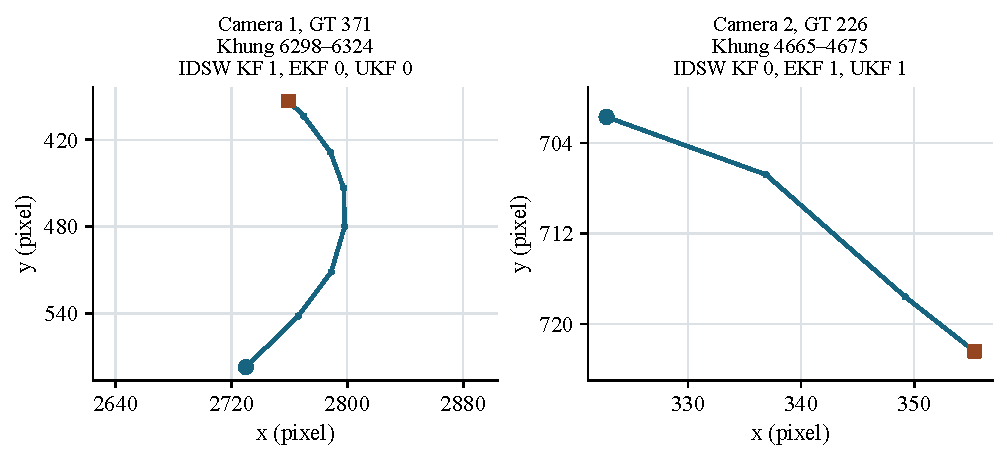
\includegraphics[width=\linewidth]{hinh/quy-dao-roundabout.pdf}
\caption{Hai đoạn đổi hướng trên RoundaboutHD. Đường biểu diễn tâm đáy hộp GT trên ảnh, với dấu tròn ở đầu và dấu vuông ở cuối. Hai ví dụ được chọn sau khi chấm để minh họa các trường hợp trái chiều.}\label{fig:trajectory-cases}
\end{figure}

Khi chấm toàn bộ 24.000 khung mới, KF có IDSW thấp nhất và HOTA cao nhất, 40,46\%. HOTA tương ứng của EKF, UKF và PF500 là 40,37\%, 40,19\% và 37,33\%. Kết quả theo nhóm rẽ mô tả các sự kiện được ghi trong lịch sử ghép liên tục. Điểm gộp toàn cửa sổ được chấm với lịch sử đánh giá bắt đầu ở khung 3.001, nên có thể lệch vài sự kiện ngay ranh giới. Toàn bộ bốn góc quay thuộc cùng một vòng xuyến. Điều này giới hạn khả năng suy rộng tỷ lệ giảm sang các nút giao độc lập.

\subsection{HELMET: theo dõi xe máy trên toàn tập test}
Tập HELMET cung cấp chuỗi phương tiện hai bánh ở 12 nhóm cảnh \cite{helmet}. Tập test chính thức chứa 182 clip, 18.200 khung, 54.529 hộp GT và 1.788 ID tính theo clip. Bộ lọc được so trên cùng cache YOLO11n mixed5 ở c10. Tại IoU 0,50 và ngưỡng điểm lớn hơn 0,10, detector đạt precision 45,17\% và recall 42,38\% cho xe máy. Hộp GT thường bao cả xe và người ngồi. Kết quả theo dõi phản ánh toàn clip theo quy tắc chú thích đó.

\begin{table}[htbp]\centering\small
\caption{So sánh trên HELMET với YOLO11n mixed5 c10. PF500 là trung bình ba seed.}\label{tab:helmet}
\begin{tabular}{@{}lrrrr@{}}\toprule
Phạm vi và chỉ số & KF & EKF & UKF & PF500\\\midrule
182 clip, IDSW & 717 & 444 & 452 & 630\\
182 clip, HOTA (\%) & 20,81 & 21,66 & 21,82 & 18,71\\
146 clip bổ sung, IDSW & 639 & 390 & 398 & 554,33\\
146 clip bổ sung, HOTA (\%) & 21,22 & 22,13 & 22,21 & 19,12\\\bottomrule
\end{tabular}
\end{table}
Trên toàn tập test, EKF giảm 38,08\% IDSW và UKF giảm 36,96\% so với KF, đồng thời HOTA tăng trên cả hai cấu hình. Mức giảm IDSW vẫn xuất hiện khi tách riêng 146 clip chưa dùng trong lượt test36. Số FN của cả bốn cấu hình còn cao, từ 43.644 đến 44.813 tùy lượt. Vì chưa phân tầng HELMET theo lúc xe đổi hướng hoặc che khuất, phép đo này hỗ trợ nhận định về giữ ID xe máy trên tập test mà chưa tách được tác động của từng kịch bản.

\subsection{UA-DETRAC: đổi ID ở các đoạn che khuất}
Phép hậu kiểm R113 dùng 40 đoạn test, mỗi đoạn 150 khung, với cùng phát hiện YOLO11n 50/50 c25 từ Jetson Nano. Mỗi lần đổi ID và mỗi hộp bỏ sót được quy về hộp GT tại khung đó sau khi phát lại lịch sử ghép CLEAR trên toàn đoạn. Phép kiểm khớp tổng IDSW và FN ở cả 120 tổ hợp đoạn và bộ lọc.

\begin{table}[htbp]\centering\small
\caption{Kết quả theo khả kiến trên 40 đoạn UA-DETRAC. Trong mỗi ô là IDSW và FN, theo thứ tự.}\label{tab:ua-occlusion-r113}
\begin{tabular}{@{}lrrrr@{}}\toprule
Phạm vi & Hộp GT & KF & EKF & UKF\\\midrule
Khả kiến $\leq 0{,}5$ & 7.486 & 53 / 4.941 & 50 / 4.940 & 48 / 4.939\\
Có che trong một giây gần nhất & 10.097 & 86 / 5.793 & 83 / 5.792 & 77 / 5.791\\
Toàn đoạn & 74.354 & 245 / 17.590 & 250 / 17.593 & 248 / 17.591\\\bottomrule
\end{tabular}
\end{table}

Trong 7.486 hộp có khả kiến thấp, EKF giảm 5,66\% và UKF giảm 9,43\% IDSW so với KF, với chênh lệch tối đa hai hộp bỏ sót. Bootstrap ghép cặp theo 40 đoạn cho khoảng phân vị 95\% của chênh lệch IDSW là $[-8,2]$ với EKF và $[-15,3]$ với UKF. Cả hai khoảng đều chứa 0. Kết quả toàn đoạn cho thứ hạng khác. Nhóm gồm xe vừa rẽ từ $25^\circ$ vừa bị che chỉ có 34 hộp, trong đó mỗi bộ lọc bỏ sót 32 hộp. Cần thêm dữ liệu hỗn hợp để kiểm chứng đồng thời xe rẽ, xe bị che và từng loại phương tiện.

\subsection{Đối chiếu đổi hướng với camera gắn xe}
Trên 40 đoạn BDD100K, nhóm đổi hướng trên ảnh từ $25^\circ$ có 2.205 hộp xe. IDSW lần lượt là 64, 61 và 59 với KF, EKF và UKF. Riêng ô tô có 1.896 hộp và IDSW 58, 56 và 54. Số bỏ sót ô tô lần lượt là 973, 977 và 978. 147 hộp xe máy trong mẫu chưa tạo đoạn đạt tiêu chí rẽ. Đây là phân nhóm theo lớp GT của phép ghép phương tiện gộp.

Hai clip METEOR \cite{meteor} được chọn theo số đoạn đổi hướng trong nhãn trước khi xem kết quả. Trong nhóm rẽ có 425 hộp ô tô và 670 hộp xe máy hoặc scooter. IDSW ô tô bằng 0 ở cả ba bộ lọc, với 294 hộp bỏ sót mỗi bộ lọc. IDSW xe máy là 2, 1 và 1, với 658 hộp bỏ sót mỗi bộ lọc. Chỉ 18 hộp xe máy rẽ có phát hiện cùng lớp đạt IoU ít nhất 0,5. Độ phủ thấp và số lần đổi ID ít giới hạn giá trị suy rộng của pilot. Cả BDD và METEOR đều đo đổi hướng trên ảnh, nên kết quả bao hàm chuyển động của camera.

\section{Chẩn đoán sai số PF trên RoundaboutHD}
Để tìm chênh lệch xuất hiện ở bước nào, nghiên cứu cố định YOLOv8n mixed5 c25 và ghi trạng thái ngay sau dự đoán, trước ghép. Với mỗi cấu hình và camera, hai đường bật và tắt ghi log phải trả cùng quỹ đạo. Cả 24 đơn vị đều trùng byte với kết quả benchmark. Các chuỗi kiểm tra trạng thái nội bộ sau dự đoán, cập nhật và các bước PF cũng trùng giữa hai đường.

Phép chẩn đoán nối đầu ra ở quan sát trước với GT bằng phép ghép một-một, loại ứng viên IoU dưới 0,5 trước khi gán, rồi theo cùng GT tới khung hiện tại. Sai số là khoảng cách tâm dự đoán đến tâm GT chia cho chiều cao hộp GT. Khoảng hai khung có chỉ số cách nhau một đơn vị tương ứng với \emph{không} có khung thiếu quan sát ở giữa. Trên 35.465 bộ camera--ID chuẩn--khung liền kề hợp lệ ở cả sáu lượt, sai số trung vị của CV là 0,063 chiều cao hộp, PF là 0,095--0,096. IoU trung vị tương ứng là 0,810 và 0,739--0,742.

\begin{table}[htbp]\centering\small
\caption{Sai số tâm trung vị theo số khung thiếu quan sát. Số đo tính trên mẫu nối được GT của từng bộ lọc. Khoảng PF là min--max của ba seed. Nguồn R65, lượt chẩn đoán thứ hai.}\label{tab:gap}
\begin{tabular}{lrrrr}\hline
Bộ lọc & 0 & 1--2 & 3--8 & Ít nhất 9\\\hline
CV & 0,063 & 0,122 & 0,274 & 0,80\\
EKF & 0,060 & 0,113 & 0,266 & 0,86\\
UKF & 0,060 & 0,114 & 0,269 & 0,86\\
PF500 & 0,097--0,098 & 0,174--0,179 & 0,524--0,533 & 1,58--1,65\\\hline
\end{tabular}
\end{table}

\begin{figure}[htbp]\centering\small
\begin{tabular}{lcll}\hline
Khung thiếu & Bộ lọc & Sai số tâm / chiều cao hộp GT & Trung vị\\\hline
0 & CV & \rule{2.52mm}{1.6mm} & 0,063\\
  & PF & \rule{3.92mm}{1.6mm} & 0,098\\[2pt]
1--2 & CV & \rule{4.88mm}{1.6mm} & 0,122\\
  & PF & \rule{6.96mm}{1.6mm} & 0,174\\[2pt]
3--8 & CV & \rule{10.96mm}{1.6mm} & 0,274\\
  & PF & \rule{21.32mm}{1.6mm} & 0,533\\[2pt]
$\geq9$ & CV & \rule{32mm}{1.6mm} & 0,80\\
  & PF & \rule{66mm}{1.6mm} & 1,65\\\hline
\end{tabular}
\caption{Sai số dự đoán trên RoundaboutHD với YOLOv8n mixed5 c25. Độ dài thanh biểu diễn trung vị trên mẫu nối được GT của mỗi bộ lọc. PF dùng seed 0. Các nhóm có thành phần mẫu khác nhau.}
\end{figure}

Ở nhóm thiếu từ ba đến tám khung, sai số PF đã xấp xỉ nửa chiều cao hộp. Trên toàn bộ mẫu hợp lệ của mỗi cấu hình, tỷ lệ có phát hiện phù hợp với GT nhưng chi phí ghép không đạt là 8,63--8,83\% với PF và 3,68\% với CV. Tỷ lệ có ứng viên khả thi nhưng ứng viên bị quỹ đạo khác lấy chỉ là 0,68--0,75\% với PF và 0,89\% với CV. Hai nhóm thất bại này có ý nghĩa khác nhau. Nhóm đầu cho thấy có xe đúng trong đầu vào nhưng hộp dự đoán và điểm phát hiện chưa đủ cho phép gán. Nhóm sau mới phản ánh cạnh tranh giữa quỹ đạo. Phần lớn mức tăng ở nhóm đầu thuộc quỹ đạo đã mất dấu.

Trên 352 ID chuẩn, số lần phân mảnh tăng từ 1.944 ở CV lên 2.262--2.323 ở PF. Số quỹ đạo được theo dõi phần lớn thời gian giảm từ 79 xuống còn 46--48. Trung vị $N_{\mathrm{eff}}/N$ trước lấy mẫu lại là 0,188 và ngưỡng 0,5 bị vượt theo chiều giảm ở gần như mọi lần cập nhật. Khi thiếu ít nhất ba khung, sai số tâm tăng nhanh hơn độ trải hạt. Đây là các quan sát cùng xuất hiện. Phép thử không thay độc lập từng yếu tố như nhiễu, số hạt hay tốc độ khung nên nguyên nhân của sự giảm điểm vẫn chưa xác định. PF còn có nhiều mẫu không nối được GT hơn CV, vì vậy sai số trên các mẫu hợp lệ có thể đánh giá thấp mức khó của PF.

\section{Đối chiếu PF với triển khai công khai}
Thư viện Python \texttt{pfilter} phiên bản 0.2.5 cung cấp một triển khai lấy mẫu quan trọng và lấy mẫu lại (SIR) \cite{pfilter}. Phép thử đưa triển khai này vào cùng bộ nối ByteTrack và giữ số hạt, CTRV, cache, phép đo và dữ liệu chấm của cấu hình PF500 K1/K2 motion2. Hai nhánh khác nhau ở cách xây dựng đề xuất từ phép đo, bước lấy mẫu lại và xử lý các tình huống suy biến. Do các chi tiết này thay đổi cùng nhau, phép đối chứng đánh giá toàn bộ cách cập nhật hạt đã tích hợp.

\begin{table}[htbp]\centering\small
\caption{Đối chiếu hai triển khai PF trên 12 clip UA-DETRAC phát triển. Giá trị là trung bình ba seed. Nguồn R108.}\label{tab:pf-public}
\begin{tabular}{lrrrr}\toprule
Cấu hình & HOTA (\%) & IDF1 (\%) & IDSW & FN\\\midrule
PF500 K1/K2 motion2 & 57,01 & 68,36 & 697,00 & 39.395,67\\
PF500 với \texttt{pfilter} & 52,68 & 60,54 & 1.359,33 & 42.983,67\\\bottomrule
\end{tabular}
\end{table}

IDSW tăng ở cả ba seed với triển khai công khai. Khóa luận giữ PF500 K1/K2 motion2 cho các phép đối chiếu gần nhất. Biến thể ghép lại quỹ đạo Lost bằng IoU trong ba khung từng giảm IDSW từ 697 xuống 525,7 trên UA-DETRAC phát triển. Khi áp dụng lên BDD val, IDSW trung bình tăng từ 6.291,3 lên 6.712,3. Khoảng ba khung tương ứng 0,12 giây ở UA-DETRAC và 0,60 giây ở BDD, có thể góp phần vào thay đổi nhưng chưa được tách thành phép kiểm riêng. Biến thể ghép lại này không được chọn cho cấu hình chính.

\section{UTUAV và giới hạn của đầu vào}
UTUAV có cảnh giao thông nhìn từ trên cao và nhãn xe máy \cite{utuav}. Phép thử dùng hai block validation B gồm 738 khung và C gồm 751 khung. Tác giả xác nhận qua thư riêng rằng video B/C có tốc độ $30000/1001$ fps và ảnh được lấy liên tiếp với stride 1. Bước thời gian là $1001/30000$ giây và bộ đệm 1,2 giây tương ứng 36 bước.

Toàn bộ 36 lượt tracking cho ba detector, hai ngưỡng và sáu lượt bộ lọc đã hoàn tất. YOLOv8n COCO có độ phủ cao nhất, nhưng cận trên recall ở IoU 0,5 và conf $>0{,}05$ chỉ là 520/29.756 hộp GT động tại B (1,75\%) và 1.107/125.005 tại C (0,89\%). Phép kiểm này không buộc ghép một-một nên chỉ dùng làm cận trên độ phủ. HOTA của mọi cấu hình không vượt 0,46 trên thang 100.

Phát hiện quá thưa hạn chế khả năng phân biệt bộ lọc. Trường \texttt{occluded} trong nhãn đều bằng 0 nên chưa dùng để phân tầng che khuất. Kết quả này cho biết giới hạn chuyển miền của ba detector trong giao thức đã chạy.



